\documentclass[12pt]{article}
\usepackage[english]{babel}
\usepackage[utf8]{inputenc} % Permite el uso de caracteres del Español
\usepackage[T1]{fontenc}
\usepackage{graphicx}
\usepackage{amsmath}
\usepackage{wrapfig}
\usepackage{enumerate}
\usepackage[top=1in, bottom=1.25in, left=1.1in, right=1.1in]{geometry}
\usepackage[dvipsnames]{xcolor}
\usepackage{subcaption}

\begin{document}

\begin{titlepage}

\newcommand{\HRule}{\rule{\linewidth}{0.5mm}} % Define un comando para las lineas horizontales

\center 
%----------------------------------------------------------------------------------------
%	Cabezera
%----------------------------------------------------------------------------------------

\textsc{\LARGE Universidad de Sonora}\\[1.5cm]
\textsc{\Large Licenciatura en Física}\\[0.5cm]
\textsc{\large Física Computacional I}\\[0.5cm]

%----------------------------------------------------------------------------------------
%	Titulo
%----------------------------------------------------------------------------------------

\HRule \\[0.4cm]
{\huge \bfseries Actividad 2 - Python y Jupyter}\\[0.4cm] % Title of your document
\HRule \\[1.5cm]
 
%----------------------------------------------------------------------------------------
%	Autor
%----------------------------------------------------------------------------------------

\begin{minipage}{0.4\textwidth}
\begin{flushleft} \large
\emph{Alumno:}\\
José Gabriel Navarro I.
\end{flushleft}
\end{minipage}
~
\begin{minipage}{0.4\textwidth}
\begin{flushright} \large
\emph{Profesor:} \\
Carlos Lizarraga Celaya
\end{flushright}
\end{minipage}\\[2cm]


%----------------------------------------------------------------------------------------
%	Fecha
%----------------------------------------------------------------------------------------
07 de Febrero de 2017

%----------------------------------------------------------------------------------------
%	Escudo
%----------------------------------------------------------------------------------------


\includegraphics[width=0.4\textwidth]{logo.png}\\
 
%----------------------------------------------------------------------------------------

\vfill % Llena el espacio de la pagina en blanco

\end{titlepage}

En el presente reporte se habla acerca de la segunda actividad realizada para la clase de Física Computacional I, el cual abarca los conceptos de Python y Jupyter, y las distintas funciones, ventajas, desventajas y bondades de estos. \\

\begin{wrapfigure}{r}{0.3\textwidth}
    \centering
    
\includegraphics[width=0.35\textwidth]{LogoP.png}
\end{wrapfigure}
\section{Introducción e Investigación}
Primeramente y como introducción, ¿qué es Python y que es Jupyter?. Python es un lenguaje de programación multiparadigma, ya que soporta orientación a objetos, programación imperativa y, en menor medida, programación funcional. Es un lenguaje interpretado, es decir, el código se escribe en un lenguaje legible por humanos y se traduce renglón por renglón, no lo compila, lo lee mientras se escribe. Posee una licencia de código abierto, denominada Python Software Foundation License y es compatible con la licencia general GNU. Una de las librerias mas usadas para el análisis de datos en Python es la llamada \textbf{panda}. Panda es un paquete de Python que provee estructuras para datos de una manera rapida y flexible, diseñado con el proposito de que sea mas fácil e intuitivo la organización de datos. Panda permite analizar datos de distintas formas, por columnas de tipo SQL o Excel, ordenados o desordenados, etcétera. Las principales formas de lectura de datos son \textbf{\textit{series}} (para datos unidimensionales) y \textbf{\textit{dataframe}} (para datos bidimencionales). \\

\begin{wrapfigure}{l}{0.4\textwidth}
    \centering
    
\includegraphics[width=0.35\textwidth]{LogoJ.png}
\end{wrapfigure}

Ahora bien, Jupyter es una aplicación web de código abierto que permite la creación y compartir documentos que contienen código, ecuaciones, visualizaciones de imagenes y texto. Soporta hasta 40 tipos distintos de lenguajes, entre ellos R y Python. En esta clase se utilizara para poder realizar análisis de datos en Python, como se mostrará mas adelante en el reporte. En el caso de esta actividad, se utilizo para el análisis de eventos climatologicos en un cierto estado del país. \\\\\\

\section{Actividades a realizar}
\subsection{Comandos principales de pandas y Python}
Antes de realizar el análisis de datos correspondiente al estado elegido, se deben importar las bibliotecas correspondientes para poder hacerlo. Estas bibliotecas son la de "panda" ya mencionada anteriormente y la de  matplotlib.pyplot, que se usa para graficar.\\

\begin{center}
\textcolor{ForestGreen} {import} pandas \textcolor{ForestGreen}{as} pd\\
\textcolor{ForestGreen} {import} numpy \textcolor{ForestGreen} {as} np\\
\textcolor{ForestGreen} {import} matplotlib.pyplot \textcolor{ForestGreen} {as} plt
\end{center}

Una vez importadas las librerías a utilizar, primeramente vamos a leer los datos del archivo del estado elegido, en este caso: Rio Tomatlan. Esto lo hacemos mediante el comando \textit{read\_csv}, indicando el nombre del archivo, los renglones que se deben saltar, y el tipo de separación que existe entre los datos, como en el archivo están separados por mas de un espacio, se usa el termino: \text{'\textbackslash s+'}. 

\begin{center}
\text {df0 = pd.read\_csv(\textcolor{red}{'RioTomatlan.txt'}, skiprows=4, sep=\textcolor{red}{'\textbackslash s+'})}
\end{center}

Para revisar si el archivo fue leído con éxito, podemos utilizar el comando \textit{df0.head()}, que mostrara los primeros cinco renglones de los datos leídos, al colocar un numero entre los paréntesis, ese es el numero de renglones que se mostraran en pantalla.

\begin{figure}[h]
    \centering
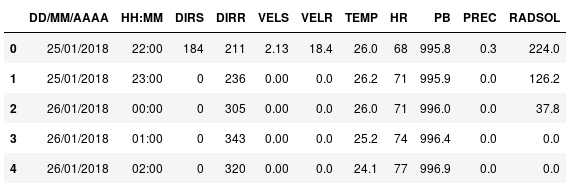
\includegraphics[width=4in]{tabla5ren.png}
\end{figure}

\begin{wrapfigure}{l}{0.3\textwidth}
    \centering
    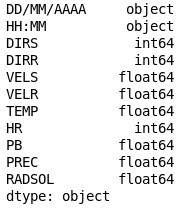
\includegraphics[width=0.25\textwidth]{TiposDatos.png}
\end{wrapfigure}

Ahora vamos a darle forma de datos, es decir, panda le dará una clasificación a cada tipo de dato que hay en el archivo. Esto se hace por medio del comando \textit{df = pd.DataFrame(df0)}, si compila bien, al introducir el código \textit{df.dtypes}, aparecerán en pantalla el tipo de datos que existe en el archivo. Como se puede observar, los que son números los toma como int64, y los que tienen punto decimal los toma como float64. Ademas de esto también aparece la clasificación de object, que es el tipo que se le pone a los datos que panda no reconoce. (Sin embargo si existe un tipo para la fecha).  \\

Para poder realizar gráficas de los datos contra el tiempo, combinaremos dos columnas, siendo estas la de fecha y hora, esto con el comando de df, seguido por el nombre de la nueva columna, en donde indicamos que tomaremos las columnas de Fecha y de Hora. Al combinarlas indicamos que el día debe de aparecer primero en el formato, ya que en el archivo viene indicado así. Ya combinadas, eliminamos las columnas de fecha y hora, esto mediante el código: \textit{df.drop}, indicando las columnas a eliminar. \\

\begin{center}
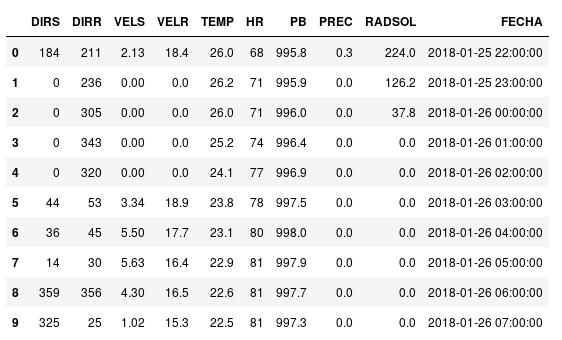
\includegraphics[scale=0.7]{NuevaTabla.png}
\end{center}
 
Además de esto, la librería de panda nos ofrece otro tipo de análisis de datos, entre ellos varios datos estadísticos, como lo es el numero de datos, la media, la desviación estándar, mínimo y máximo y los cuartiles. Se puede dar un análisis general de todos los datos con el comando \textit{df.describe()}. Sin embargo, si se desea un análisis especifico de todos los datos, o un análisis especifico de un dato en especifico, podemos utilizar \textit{df.DATO.VALOR}, donde dato es el dato en especifico y valor el valor en especifico, o también puede pedirse entre un rango de valores utilizando \textit{df\_select}, por ejemplo: \\

\begin{figure}[h!]
\begin{subfigure}{.5\textwidth}
  \centering
  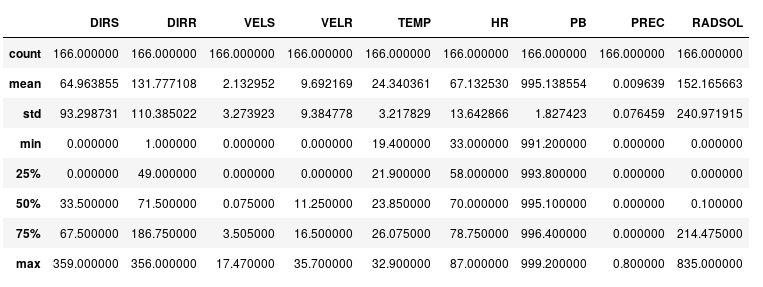
\includegraphics[width=.8\linewidth]{Estad1.png}
  \caption{Un análisis general de los datos}
  \label{fig:sfig1}
\end{subfigure}%
\begin{subfigure}{.5\textwidth}
  \centering
  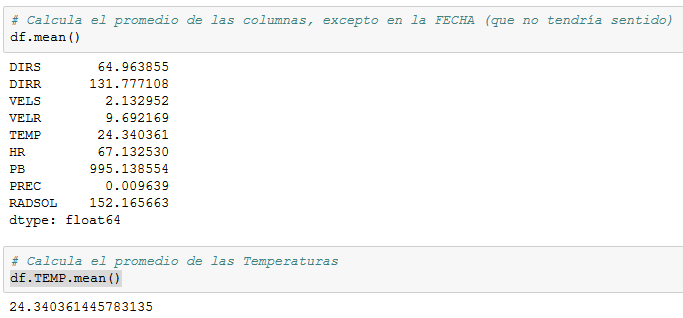
\includegraphics[width=.8\linewidth]{Estad2.png}
  \caption{Análisis de una medida en especifica.}
  \label{fig:sfig2}
\end{subfigure}
\end{figure}

El paquete de matplot, permite la realización de gráficas, y para utilizarlo solamente se debe usar el comando \textit{plt.figure}, en donde se indica que es lo que se va a graficar y contra quien, en donde se puede especificar también el nombre del gráfico, así como el nombre de sus ejes, plt.grid indica que si se desea usar la cuadricula de fondo y plt.show muestra la gráfica en pantalla: 

\begin{center}
plt.figure(); df.RAPVIENTO2.plot(); plt.legend(loc='best') \\
plt.title(\textcolor{red}{"Variación de la Rapidez de los Vientos"})\\
plt.ylabel(\textcolor{red}{"Rapidez (m/s)"})\\
plt.grid(\textcolor{ForestGreen}{True})\\
plt.show()\\
\end{center}

También se puede escoger en especifico que dato va en cada eje, para de esta manera realizar cualquier gráfica que se desee. Además, se puede cambiar el formato de la gráfica, como lo es su color. Esto lo podemos hacer en la linea de código: \textit{plt.plot\_date(x=df.DATO, y=dfDATO., fmt="COLOR-")}, en donde DATO es la columna de DATOS a utilizar y COLOR la primera letra del color que queremos. \\

Con estas herramientas, podemos realizar análisis de datos muy extensos, facilitando mas así nuestro trabajo. A continuación se responden las preguntas correspondientes a la practica.

\begin{figure}[h!]
\begin{subfigure}{.5\textwidth}
  \centering
  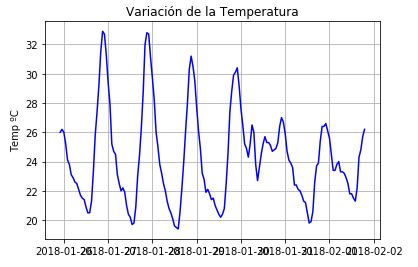
\includegraphics[width=.8\linewidth]{EjGraf1.png}
  \caption{Gráfica de la Variación de la Temperatura}
  \label{fig:sfig1}
\end{subfigure}%
\begin{subfigure}{.5\textwidth}
  \centering
  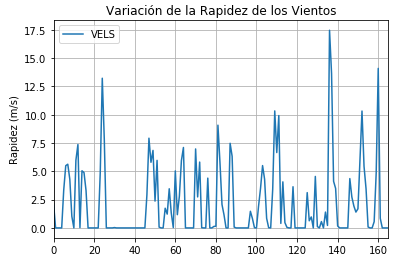
\includegraphics[width=.8\linewidth]{EjGraf3.png}
  \caption{Gráfica de la variación de la rapidez de los vientos}
  \label{fig:sfig2}
\end{subfigure}
\end{figure}


\newpage

\subsection{Analisis de Datos de Río Tomatlan}
\noindent\textbf {1. Crear una gráfica que muestre la rapidez de los vientos y la rapidez de las ráfagas, como funciones del tiempo. ¿Cuáles son las horas del día con más viento?} \\

\begin{wrapfigure}{l}{0.57\textwidth}
    \centering
    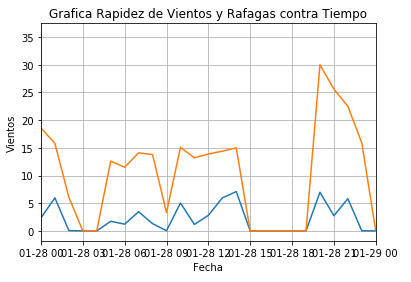
\includegraphics[width=0.6\textwidth]{ViRa.png}
\end{wrapfigure}

Para el análisis de velocidad de ráfagas y vientos, se eligió el rango entre los días 28 de enero de 2018 y 29 de enero de 2018. Como se puede observar en la gráfica existen varios registros de ciertos picos en la velocidad del viento y ráfagas, siendo en el rango de 20:00 a 00:00 horas en donde, tanto como la velocidad de los vientos, como de las ráfagas era el mayor en ese día. Además de esto, se puede observar como en las tardes no hay mucho viento.\\


\noindent\textbf {2. Crear una gráfica con la dirección de los vientos como función del tiempo y comentar sobre los vientos dominantes en el sitio de estudio.} \\

\begin{wrapfigure}{r}{0.57\textwidth}
    \centering
    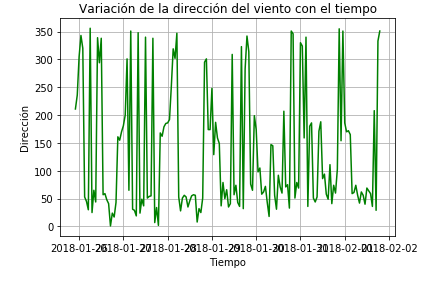
\includegraphics[width=0.7\textwidth]{DirVi.png}
\end{wrapfigure}

La siguiente gráfica muestra el comportamiento de la dirección de los vientos durante 5 días, en donde como se puede observar, la mayoría de las veces o llegan hasta casi los 360$^{\circ}$, pero en otras horas del día llegan a casi 0$^{\circ}$. Este patrón se puede observar sobre todo entre las ultimas horas del día y las primeras horas del siguiente día, en donde los vientos son dirigidos hacia el sur, mientras que en las tardes, los vientos están dirigidos hacia el norte/noroeste.\\ \\ \\ \\ \\ \\


\noindent\textbf {3. Muestre el comportamiento de la Radiación Solar como función del tiempo. ¿Qué puedes comentar? } \\

Se puede observar varios registros con 0, esto se debe a que en esas horas aun es de noche, por tanto no hay Sol, y pues no hay radiación solar. Otra cosa a notar es que existen días con mucha radiación solar, siendo los primeros días lo que llegan hasta casi 800, mientras que los últimos días llegan hasta 300.

\begin{center}
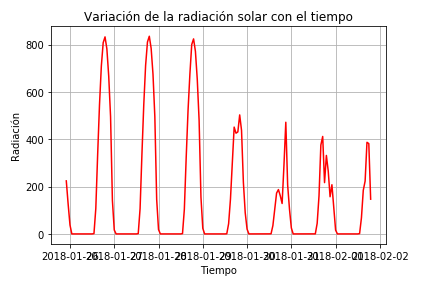
\includegraphics[scale=0.65]{RadSol.png}
\end{center}

\noindent\textbf {4. ¿Cuál es el lapso de temperatura diaria? (Diferencia entre la temperatura máxima y la mínima). } \\

Se tomara el mismo rango de días que se tomo para el análisis de vientos y ráfagas, es decir del 28 de enero de 2018 y al 29 de enero de 2018.\\

Para esta evaluación, se creo otro dataframe con solo las temperaturas dentro del rango indicado, como se muestra en la figura. 

\begin{center}
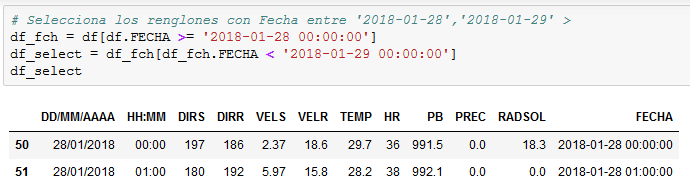
\includegraphics[scale=0.65]{Nuevodf.png}
\end{center}

Entonces, ahora con el nuevo dataframe, calculamos el maximo, el minimo, y los restamos, obteniendo que el lapso es de 11.8. 

\begin{center}
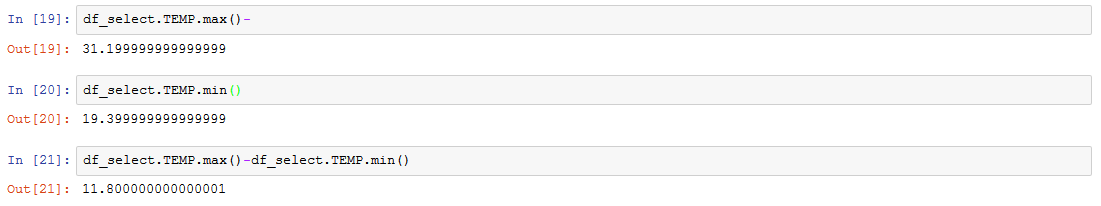
\includegraphics[scale=0.6]{diferencia.png}
\end{center}

\noindent\textbf {5. ¿Puedes comentar sobre la relación entre la temperatura y la humedad relativa?} \\

\begin{wrapfigure}{r}{0.57\textwidth}
    \centering
    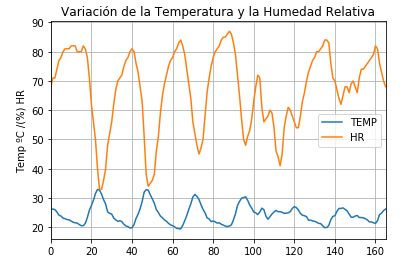
\includegraphics[width=0.6\textwidth]{VarTempHum.png}
\end{wrapfigure}

Como se puede observar por la grafica, la temperatura cambia entre un rango de 32$^{\circ}$-18$^{\circ}$, sin embargo, el cambio de la humedad es muy grande en los intervalos de tiempo, como se puede observar varia mucho, desde 80$^{\circ}$ hasta casi 32$^{\circ}$. \\ 

Cuando la temperatura es muy baja, la humedad es alta, y cuando la temperatura es alta, la humedad es baja. \\ \\

\noindent\textbf {6. Realiza el análisis exploratorio de datos, que resuma el sitio estudiado (Usar la función describe() sobre tu data frame. } \\

A continuación se muestra el análisis exploratorio de los datos de Río Tomatlan:

\begin{center}
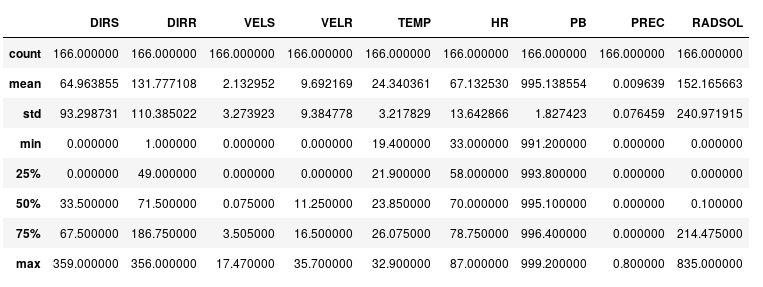
\includegraphics[scale=0.6]{Estad1.png}
\end{center}

\section{Apéndice}
\noindent\textbf {1. ¿Cuál es tu primera impresión de Jupyter Notebook?}\\\\
Es un entorno muy interesante de programación, me recordó mucho a cuando en mi preparatoria usábamos un servidor local en el navegador para crear bases de datos dinámicas, solo que este entorno es mas limpio y en realidad se programa, sin mencionar que la librería panda es muy buena para el análisis de datos. \\ \\

\noindent\textbf {2. ¿Se te dificultó leer código en Python?}\\ \\
Al iniciar si se me dificulto un poco, ya que no tenia experiencia alguna con este lenguaje de programación. Pero revisando e investigando las distintas funciones que presenta panda y Python, además de la ayuda del profesor y compañeros, al realizar las preguntas respecto al estado y ciudad seleccionada, fue fácil. \\ \\

\noindent\textbf {3. ¿En base a tu experiencia de programación en Fortran, que te parece el entorno de trabajar en Python?} \\ \\
Siento que los comandos e instrucciones de Fortran son mas claros en lo que hacen, pero la sintaxis y forma de trabajo de Python son mucho mejor. El lenguaje Fortran es de compilación, mientras que Python es de interpretación, lo cual siempre he encontrado (en mi opinión) que es mejor. \\ \\

\noindent\textbf {4. A diferencia de Fortran, ahora se producen las gráficas utilizando la biblioteca Matplotlib. ¿Cómo fue tu experiencia?.} \\ \\
Graficar es mucho mas facil en Python que en Fortran. En Fortran se tenia que generar los datos, para posteriormente introducirlos a GNUPlot, y en veces este no hacia lo que se le pedia, a pesar de no tener errores al declarar la grafica. Python, en caso de tener un error, lo muestra y es claro en ello. \\ \\

\noindent\textbf {5 .En general, ¿qué te pereció el entorno de trabajo en Python?} \\ \\
Es muy interesante y limpio, la facilidad de poder parar un proceso en caso de ser erróneo es algo grandioso, además de que con la experiencia anterior que tengo de programación, Python es de los lenguajes mas fáciles de manejar que he tenido la oportunidad de usar.  \\ \\

\noindent\textbf {6. ¿Qué opinas de la actividad? ¿Estuvo compleja? ¿Mucho material nuevo? ¿Que le faltó o que le sobró? ¿Qué modificarías para mejorar?} \\ \\
Al comenzar la actividad, pensé que era demasiado material nuevo, pero eso se debia a mi poca experiencia con el lenguaje. Una vez trabajando en ello me di cuenta que en realidad son los usos básicos de Python, análisis de datos y graficas. La practica fue una muy buena introducción al entorno de Python y su uso. \\ \\

\noindent\textbf {7. ¿Comentarios adicionales que desees compartir?} \\ \\
Esa practica fue una muy buena introducción al entorno de Python y sus funciones, ademas de su ambiente de Jupyter. \\ \\

\section{Bibliografía}
\begin{itemize}
    \item Kumar, Nikhil. Graph Plotting in Python. Recuperado de: www.geeksforgeeks.org/graph-plotting-in-python-set-1/
    \item Quintero, Francisco (2012, Septiembre 2). Lenguajes de Programación. Recuperado de: otroespacioblog.wordpress.com/2012/09/02/lenguajes-de-programacion-compilados-vs-interpretados/
    \item Python. (2018, Febrero 4). Recuperado de: https://en.wikipedia.org/wiki/\\Python\_(programming\_language)
\end{itemize}

Imagenes utilizadas: 
\begin{itemize}
    \item Simbolo Jupyter: Fecha: Agosto 2017, https://gitlab.eurecom.fr/zoe-apps/zapp-jupyter/\\blob/master/logo.png
    \item Simbolo Python: https://www.python.org/community/logos/ 
\end{itemize}

\end{document}
